\documentclass[12pt]{article}
% pre\'ambulo
\usepackage{lmodern}
\usepackage[T1]{fontenc}
\usepackage[spanish,activeacute]{babel}
\usepackage{mathtools}
\usepackage{amsmath}
\usepackage{amssymb}
\usepackage{url}
\usepackage{tikz}
\usepackage{graphicx}
\usepackage{algorithm}
\usepackage[noend]{algpseudocode}
\graphicspath{ {images/} }
\usetikzlibrary{arrows,positioning}
\tikzset{
    %Define standard arrow tip
    >=stealth',
    %Define style for boxes
    punkt/.style={
           rectangle,
           rounded corners,
           draw=black, very thick,
           text width=5em,
           minimum height=4em,
           text centered},
    % Define arrow style
    pil/.style={
           ->,
           thick,
           shorten <=2pt,
           shorten >=2pt,}
}
\usepackage[style=numeric-comp,backend=bibtex]{biblatex}
\bibliography{refs.bib}

\title{Dise\~no y verificaci\'on formal de programas moleculares en el modelo d\'ebil de Amos}
\author{Sergio Rodr\'iguez Calvo}
\date{Septiembre de 2017}


\begin{document}
    \maketitle
    \thispagestyle{empty}
    \begin{center}
      Departamento de Ciencias de la Computaci\'on e
      Inteligencia Artificial \\
      Universidad de Sevilla
      \end{center}
  % cuerpo del documento
  % abstract
  \bf{Abstract. }\rm
    \emph{En el presente trabajo se pretende estudiar el dise'no y la verificaci'on formal
    de dos programas moleculares en el modelo d'ebil de Amos que resuelven el problema de la generaci'on
    de permutaciones; y el problema del camino hamiltoniano en su versi'on dirigida y sin
    nodos distinguidos. En concreto, se centra en reescribir, as'i como, completar algunos detalles
    de las demostraciones, que se encuentran el trabajo original \cite{Mario-deJesus}.
    El desarrollo de este trabajo tiene como objetivo ser entregado como trabajo final de la asignatura de
    Computaci'on Bioinspirada.}

\section{Introducci'on}

En la d'ecada de los cincuenta comienza a ser evidente que existe una analog'ia entre algunos procesos
matem'aticos y ciertos procesos biol'ogicos. Un organismo vivo puede ser visto como el resultado de
aplicar una serie de operaciones bioqu'imicas sobre una cadena de 'acido desoxirribonucleico (ADN).

Posteriormente, en la decada de los noventa, se demostr'o que se pueden usar ciertos procesos biol'ogicos
para atacar la resolubilidad de problemas matem'aticos dif'iciles. Estos problemas tambi'en son conocidos
como computacionalmente intratables, y son aquellos que su soluci'on algor'itmica toma una cantidad de
recursos exponenciales en el tama'no del dato de entrada.

Esta resolubilidad est'a relacionada con la potencia de c'alculo y la densisdad de almacenamiento de los
ordenadores convencionales.

En la propia d'ecada de los cincuenta ya se introdujo el concepto te'orico de computaci'on a nivel molecular.
En los ordenadores convencionales la paralelizaci'on y la miniturizaci'on son un objetivo importante, y la
computaci'on molecular puede suponer un paso m'as en este sentido.

Sobre todo, a partir de que en la d'ecada de los ochenta cuando se demostr'o la existencia un l'imite en la potencia
de c'alculo y en la miniturizaci'on de los componentes electr'onicos empleados en los ordenadores convencionales.

Por 'ultimo se enumeran las principales ventajas del uso de la computaci'on molecular:

\begin{itemize}
	\item Sustituci'on de la luz por reacciones qu'imicas, lo que implica un ahorro del consumo energ'etico.
	\item El uso de interruptores moleculares permite, seg'un se estima, disponer de m'as de mil procesadores
    en el mismo espacio que un procesador convencional.
	\item Se estima que los interruptores moleculares pueden aumentar cien mil millones de veces la capacidad
    de procesamiento respecto a los ordenadores convencionales.
	\item Se estima que se podr'ian reproducir la capacidad de cien ordenadores en el tama'no de un grano de sal fina.
\end{itemize}

\section{Modelo d'ebil de Amos}

Antes de introducir el Modelo d'ebil de Amos, se necesita previamente conocer los detalles y principios
de la computaci'on molecular, as'i como, los distintos modelos previos a este, los cuales se pueden encontrar
en el documento original del profesor del departamento de Ciencias de la Computaci'on de la Universidad
de Sevilla, Mario de Jes'us P'erez Jim'enez \cite{Mario-deJesus}.

El Modelo d'ebil de Amos consiste en modelo de computaci'on basada en ADN, esto es, que utiliza como sustrato
computacional el ADN y en el cual se realizan filtrados sobre el sustrato anterior. En este caso, no existe
memoria de acceso aleatorio como en la computaci'on cl'asica. Para almacenar el sustrato, al igual que en otros
modelos de computaci'on molecular, se utiliza un tubo de ensayo que contendr'a la muestra.

Dicho tubo es un multiconjunto finito de cadenas del alfabeto $\sum_{ADN} = \{A, C, G, T\}$.

A nivel abstracto, en el Modelo d'ebil de Amos las operaciones que se pueden realizar sobre los tubos
son las siguientes:

\begin{itemize}
    \item \textbf{Quitar (\textit{T},\{$ \gamma_{1},...,\gamma_{n} $\}):} Dado un tubo, \textit{T}, y un n'umero finito
    de cadenas, $ \gamma_{1},...,\gamma_{n} $, de $ \sum $, devuelve el tubo obtenido de T eliminando
    todas aquellas cadenas que contengan, al menos, una ocurrencia de alguna de las cadenas
    $ \gamma_{1},...,\gamma_{n} $.
    \item \textbf{Copiar (\textit{T},\{$ \textit{T}_{1},...,\textit{T}_{n} $\}):} Dado un tubo, \textit{T}, y un numero
    natural $ \textit{k} \geq 2 $, devuelve \textit{k} tubos, $\textit{T}_{1},...,\textit{T}_{n}$, que son
    copias exactas de \textit{T}.
    \item \textbf{Uni'on (\{$ \textit{T}_{1},...,\textit{T}_{n} $\}):} Dados los tubos
    $\textit{T}_{1},...,\textit{T}_{n}$, con $ \textit{k} \geq 2 $, devuelve un tubo \textit{T}, cuyo contenido
    es la uni'on de los tubos $\textit{T}_{1},...,\textit{T}_{n}$ como multiconjuntos.
    \item \textbf{Selecci'on (\textit{T}):} Dado un tubo, \textit{T}, selecciona aleatoriamente un elemento de \textit{T}
    en el caso en que $\textit{T} \neq \emptyset$; en caso contratio, devuelve \textbf{NO}.
\end{itemize}

Estas operaciones ser'an instrucciones moleculares primitivas del modelo d'ebil. Adem'as, cabe destacar que
en este modelo la 'unica operaci'on molecular que implementa paralelismo masico es \textit{quitar}.

El primer problema, el de la generaci'on de permitaciones, ser'a abordado previo al problema del camino hamiltoniano
, ya que, ser'a necesario para su resoluci'on.

\subsection{Problema de la generaci'on de permutaciones}

En esta secci'on se muestra como abordar desde el punto de vista de la computaci'on molecular la resolubilidad
del problema de la generaci'on de permutaciones. Antes, se define en qu'e consiste una permutaci'on para a
continuaci'on abordar el problema de la generaci'on de las mismas.

Una permutaci'on la definimos como \textit{dado un numero natural, $n \geq 1$, una permutaci'on de orden n es una
aplicaci'on biyectiva del conjunto finito \{1,...,n\} en s'i mismo}.

\begin{figure}[h]
\centering
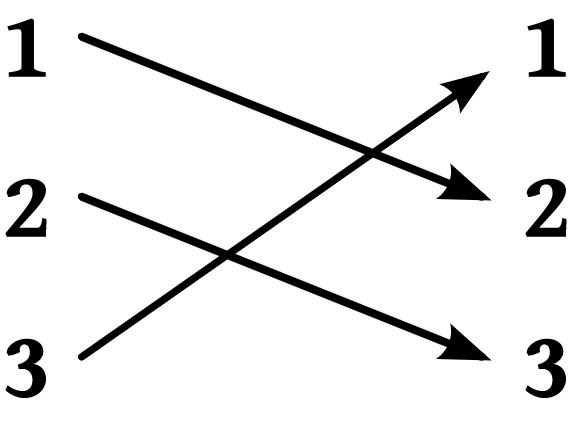
\includegraphics[scale=0.6]{permutaciones}
\caption{Ejemplo de permutaci'on considerada como funci'on biyectiva. En este caso, para $n = 3$.}
\end{figure}

Una vez tenemos definido qu'e es una permutaci'on vamos a introducir el problema de generaci'on de
permutaciones, que consiste en, \textit{dado un n'umero natural, $n \geq 2$, generar todas las permutaciones
 de orden n}.

En primer lugar, hay que definir el modelo mediante el cual se pretende representar el problema con los
elementos que tenemos en la computaci'on molecular. Esto es, definir por un lado el alfabeto:
$ \sum = \{(p_{i},c_{j}) : 1 \leq i,j \leq n\} $, donde $p_{i}$ y $c_{j}$ son dos oligos que codificar'an
respectivamente la posici'on $i$-'esima en la permutaci'on y el n'umero \textit{j}.

A continuaci'on, se necesita definir el tubo de entrada, $T_{0}$, para poder comenzar el experimento, es decir,
aplicar las operaciones abstractas de la secci'on anterior seg'un un determinado algoritmo. En este caso,
use trata de un multiconjunto de entrada con un n'umero finito de moleculas y que codifican todas las
posibles sucesiones para una longitud \textit{n}. Formalmente ser'ia:

\begin{equation*}
  T_{0} = \{\{ \sigma \in \sum_{}^n : \exists x_{1},..., \exists x_{n} (\sigma = (p_{1},x_{1}),
  (p_{2},x_{2}),..., (p_{n},x_{n})) \}\}
\end{equation*}

En la f'ormula anterior, $ \sigma $, es una codificaci'on concreta, tal que,
$ \sigma = p_{1}x_{1}...p_{n}x_{n} $.

La idea aqu'i es generar todas las posibles permutaciones, utilizando un tubo inicial, $ T_{0} $,
que contiene la codificaci'on de todas las posibles soluciones de longitud $ n $. El programa sigue los
 siguientes pasos hasta $ n - 1 $ veces:

 \begin{itemize}
     \item Un primer filtro sobre $ T_{0} $ para seleccionar las moleculas, $ \sigma $, tal que:
        \begin{equation*}
            \forall r > 1 ( (\sigma)_{1} \neq (\sigma)_{r} )
        \end{equation*}
           Esto es, para todas las posiciones, $r$, mayores que 1, devolver todas aquellas codificaciones, tal que,
           el n'umero que ocupa la posici'on $r$-'esima sea distinto de el n'umero de la primera posici'on.
     \item Un segundo filtro respecto del paso anterior donde se seleccionan las moleculas, $ \sigma $, tal que:
     \begin{equation*}
         \forall r > 2 ( (\sigma)_{1} \neq (\sigma)_{r} \land (\sigma)_{2} \neq (\sigma)_{r} )
     \end{equation*}
           Esto es, del conjunto resultante del paso anterior, para todas las posiciones, $r$, mayores que dos,
           devolver todas aquellas codificaciones, tal que, el n'umero que ocupa la posici'on $r$-'esima sea distinto
            de el n'umero de la posici'on primera y de la posici'on segunda a la vez.
 \end{itemize}}

 La notaci'on, $ (\sigma)_{r} $, representa el n'umero que ocupa la posici'on \textit{r-'esima} en la
 sucesi'on de longitud $ n $ codificada por $ \sigma $. Es decir, $ (\sigma)_{r} = x_{r} $ para todo $ r $
 $ (1 \leq r \leq n) $.

\subsubsection{Dise'no del programa molecular}

El algoritmo a seguir en el programa molecular, basado en la idea de filtrar sobre un determinado tubo $ T_{0} $
de entrada, es el siguiente:

\begin{algorithmic}
    \Require $T_{0}$
    \For {$j\leftarrow1$ in $n - 1$}
        \State copiar($T_{0}, \{T_{1},...,T_{n}\}$)
        \For {$i\leftarrow1$ in $n$}
            \State quitar($T_{i}, \{p_{j}r : r \neq i\} \cup \{p_{k}i : j + 1 \leq k \leq n\} $)
        \EndFor
        \State uni'on($\{T_{1},...,T_{n}\},T_{0}$)
    \EndFor
    \Return $T_{0}$
\end{algorithmic}

Este algoritmo presenta una complejidad $O(n^2)$, es decir, orden cuadr'atico en $n$. Por tanto, el n'umero de
operaciones moleculares es $n^2$.

\subsubsection{Verificaci'on formal del programa molecular}

Para realizar la verificaci'on formal es necesario etiquetar cada uno de los tubos que se van a obtener
a los largo del algoritmo descrito anteriormente. Por tanto, el algoritmo va a ser reescrito de la
siguiente forma:

\begin{algorithmic}
    \Require $T_{0}$
    \For {$j\leftarrow1$ in $n - 1$}
        \State copiar($T^{j-1}_{0}, \{T^{j}_{1},...,T^{j}_{n}\}$)
        \For {$i\leftarrow1$ in $n$}
            \State $\bar{T}^{j}_{i}$ \leftarrow quitar($T^{j}_{i}, \{p_{j}r : r \neq i\} \cup \{p_{k}i : j + 1 \leq k \leq n\} $)
        \EndFor
        \State uni'on($\{\bar{T}_{1},...,\bar{T}_{n}\},T^{j}$)
    \EndFor
    \Return $T_{n - 1}$
\end{algorithmic}

Antes de continuar, hay que aclarar la notaci'on a emplear a partir de aqu'i. $A_{\sigma,j}$ ser'a el conjunto
$\{\sigma_{1},...,\sigma_{j}\}$, es decir, n'umero en cada posici'on $j$-'esima, para $(1 \leq j \leq n)$, en cada
$\sigma \in T_{0}$. Esto es, un conjunto que contiene todos los n'umeros que contienen una determinada codificaci'on, $\sigma$,
desde 1 hasta la posici'on j en cada caso.

Esta notaci'on que se acaba de describir ser'a necesaria para la correci'on formal del programa que se
acaba de reescribir, y que se utiliza en la siguiente formula:

\begin{equation*}
  \theta(j) \equiv \forall \sigma \in T^{j} (|A_{\sigma,j}| = j \land \forall r ( j + 1 \leq r \leq n \rightarrow
  (\sigma)_{r} \notin A_{\sigma,j} ))
\end{equation*}

La formula, $\theta(j)$, expresa que toda molecula del tubo $T^{j}$ codifica una sucesi'on de longitud $n$ tal que
los $j$ primeros t'erminos son distintos entre s'i y, adem'as, distintos de los restantes t'erminos de la sucesi'on.

A continuaci'on, se van a exponer una serie de teoremas con los que se pretende realizar la verificaci'on formal,
tomando el algoritmo que se ha reescrito en este apartado.

\textbf{Teorema 1.1.} $\forall j (1 \leq j \leq n-1 \to \theta(j))$. Es decir, la formula $\theta$ es un invariante del
bucle principal. Esto es, que $\theta$ no cambia a lo largo de las transformaciones que sufre el tubo en el bucle principal. 

\subsection{Problema del camino hamiltoniano en versi'on dirigida sin nodos distinguidos}

El problema del camino hamiltoniano en su versi'on dirigida y sin nodos distinguidos consiste en
dado un grafo dirigido, determinar si existe un camino simple que pasa por todos los nodos del grafo. O lo
que es lo mismo, si el grafo posee un ciclo hamiltoniano.

% bibliography
\printbibliography

\end{document}
